% Copyright (c) 2021-10-07 Eclipse Arrowhead Project
%
% This program and the accompanying materials are made available under the
% terms of the Eclipse Public License 2.0 which is available at
% http://www.eclipse.org/legal/epl-2.0.
%
% SPDX-License-Identifier: EPL-2.0

We, the Eclipse Arrowhead project, here present and authoritative set of Arrowhead concept definitions, meant to serve as the foundational language for discussions about and the modelling of Arrowhead-based designs.
The document exists to help mitigate compatibility and consistency issues in software, tooling, models and all other things of relevance to Arrowhead.
The concepts established here are not specified in terms of any particular modelling tools or languages, but should be useful as foundation for any other Arrowhead modelling or documentation effort.

The description of Arrowhead we present here should be seen as an extension of \textit{Reference Architecture Model Industrie 4.0} (RAMI4.0) \cite{adolphs2016reference}.
This means that we take key concepts from RAMI4.0 and present them here in the context of the Arrowhead framework.
As RAMI4.0 is defined partly in terms of \textit{Service-Oriented Architecture} (SOA), we also builds upon \textit{Reference Model for Service Oriented Architecture} (SOA-RM) \cite{mackenzie2006reference}.
In other words, this document assumes a world-view of service-oriented communication in an Industry 4.0 setting.
This world-view is introduced more fully in Section \ref{sec:arrowhead}.

\subsection{Primary Audiences}
\label{sec:introduction:audiences}

This document is being written and maintained with the following primary audiences in mind:

\begin{itemize}
\item \textit{System architects, integrators and developers} designing, integrating or developing Arrowhead systems.
\item \textit{Standardization engineers and researchers} seeking to extend, analyze or improve upon Arrowhead.
\item \textit{Decision makers, users and other stakeholders} that need to understand fundamental Arrowhead concepts.
\end{itemize}

Those seeking a less technically rigorous description of Arrowhead may want to focus their reading on Section \ref{sec:arrowhead}.
Others are advised to read all sections carefully, in the order they are presented.

\subsection{Scope}
\label{sec:introduction:scope}

This document outlines a \GlossaryHyperRef{model-reference}{\textit{reference model}}.
We understand such to be a set of definitions for technical concepts of fundamental importance to a specific problem domain.
It does not specify how its definitions should be used to design systems, either abstract or concrete.
In the context of this document, the problem domain in question must be understood to be \textit{the design of service-oriented Industry 4.0 systems}.

Reference models can be used as vocabularies for defining \GlossaryHyperRef{architecture-reference}{reference architectures}, which in turn can be used to derive \GlossaryHyperRef{architecture}{concrete architectures} and, finally, \GlossaryHyperRef{implementation-software}{software implementations}, as illustrated in Figure \ref{fig:model-implementation-hierarchy}.

\vspace*{\fill}

\begin{figure}[ht]
  \centering
  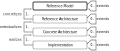
\includegraphics{figures/model-implementation-hierarchy}
  \caption{
    The hierarchical levels comprising the steps from reference models to their software implementation, going from highly abstract to entirely concrete.
    Reference models define fundamental concepts, reference architectures add abstracts limits to how they may be used together, concrete architectures makes those limits practically realizable, while implementations represent their actual realization.
  }
  \label{fig:model-implementation-hierarchy}
\end{figure}

\subsection{Notational Conventions}
\label{sec:introduction:conventions}

The following conventions regarding diagrams, references and requirements are adhered to throughout this document.
All three of them were selected by virtue of being deemed unsurprising to our primary audiences.

\subsubsection{Diagrams}

A box with a name inside it denotes a named \GlossaryHyperRef{entity}{entity}.
A named arrow between boxes denotes the \GlossaryHyperRef{relationship}{relationship} implied by the name.
If a named arrow has an associated positive integer or range, the relation is to be considered as extending to the number of distinct entities indicated by that integer or range.
A range is denoted by $x..y$, where $x$ and $y$ are positive integers and $x<y$.
Omitting $y$ when using the range notation means that the range is infinite from $x$.
A box being inside another box means that it is owned by the containing box.
See Figure \ref{fig:model-implementation-hierarchy} for an example of this graphical notation being used.

Note that this document does \textit{not} define an Arrowhead profile for SysML \cite{omg2019sysml}, or any other modelling language.
The concepts outlined here should corrsepond to the entities and relations defined by any such profiles, however.

\subsubsection{References}

Square brackets around numbers (e.g. \cite{delsing2017iot}) are references to the reference list in Section \ref{sec:references}.
The number within the brackets of any given reference corresponds to the entry with the same number in the reference list.

References within this document are hyperlinked, which means that those reading it electronically can click the references and immediately be taken to their reference targets.
Special treatment is given to references targeting Section \ref{sec:glossary}, the \nameref{sec:glossary}.
These are displayed as regular text rendered with blue color.

\subsubsection{Requirements}

Use of the words \textbf{must}, \textbf{must not}, \textbf{required}, \textbf{should}, \textbf{should not}, \textbf{recommended}, \textbf{may}, and \textbf{optional} are to be interpreted as follows when used in this document: \textbf{must} and \textbf{required} denote absolute requirements that must be adhered to for a described entity to be considered as compliant to this reference model; \textbf{must not} denotes an absolute prohibition; \textbf{should}, \textbf{should not} and \textbf{recommended} denote recommendations that should be deviated from only if special circumstances make it relevant; and, finally, \textbf{may} and \textbf{optional} denote something being truly optional.
These word definitions are derived from and are meant to capture what is outlined in RFC 2119 \cite{bradner1997keywords}.

\subsection{Relationships to Other Documents}
\label{sec:introduction:relationships}

The reference model outlined in this document is based on the following works, in order of precedence:

\begin{enumerate}
\item \textit{RAMI4.0} \cite{adolphs2016reference}, which outlines an ontological and architectural view of Industry 4.0.
As RAMI4.0 is a reference \textit{architecture} rather than a reference \textit{model}, however, its 5\textsuperscript{th} section is disregarded and its remaining sections treated as if being a reference model.
This delimitation excludes the ``architectural layers'', ``life-cycle \& value-stream'' phases and ``hierarchical levels'' of RAMI4.0.
These excluded aspects are neither condemned nor endorsed by this document.
They are simply outside its scope. 

\item \textit{SOA-RM} \cite{mackenzie2006reference}, which provides a standardized definition of SOA.
While RAMI4.0 does not include SOA-RM in its reference list, it does mention the standard and requires that all communications adhere to SOA principles. 

\item \textit{IoT Automation: Arrowhead Framework} (IoTA:AF) \cite{delsing2017iot}, which significantly includes an overview of the \textit{local automation cloud} concept in its second chapter, as well as the \textit{Arrowhead framework architecture} in its third chapter.
While the strictly architectural aspects of IoTA:AF are out of scope, the two chapters contain several definition with a high degree of relevance to this document.

\end{enumerate}

You are not assumed to have read any of the above documents prior to reading this.
Concepts derived from the above sources are reiterated in this document as necessary.

\newpage

\subsection{Section Overview}
\label{sec:introduction:sections}

The remaining sections of this document are organized as follows:
\vspace*{2mm}
\begin{itemize}[leftmargin=2cm,rightmargin=0pt,labelwidth=2cm,labelsep=0pt,itemindent=0pt,parsep=0.1cm,topsep=0.1cm,align=left]

%\item[Section \ref{sec:introduction}]
%This section.

\item[Section \ref{sec:arrowhead}]
An informal overview of Arrowhead, serving both to provide a workable summary of the framework and to prepare readers for better understanding Section \ref{sec:model}.

\item[Section \ref{sec:model}]
The formal and normative description of Arrowhead.

\item[Section \ref{sec:conformance}]
A brief list of requirements, meant to help determine whether or not a given system is conforming to this document.

\item[Section \ref{sec:glossary}]
Lists all significant terms referred to or defined in this document in alphabetical order.

\item[Section \ref{sec:references}]
Lists references to publications referred to in this document.

\item[Section \ref{sec:revision}]
Records the history of changes made to this document.

\end{itemize}
